\documentclass{jlreq}
\usepackage[dvipdfmx]{graphicx}
\usepackage[dvipdfmx]{color}
\usepackage[dvipdfmx]{hyperref}
\usepackage{amsmath}
\usepackage{geometry}
\usepackage{float}
\usepackage{array}
\usepackage{caption}
\usepackage{hyperref}
\usepackage{url}
\linespread{1.2}
\numberwithin{equation}{section}
\counterwithin{figure}{section}
\counterwithin{table}{section}
\ModifyHeading{section}{before_space=30pt, after_space=20pt}
\ModifyHeading{subsubsection}{before_space=20pt, after_space=20pt}

\begin{document}

\section{目的}
回路シミュレータSPICEの原理を理解し、シミュレーション結果と測定結果の比較を行うことで回路に対する知識を広げ、SPICEの扱いに慣れる。また、プログラムで回路方程式を解くことと、実際に数値積分公式を利用することで回路方程式に対する数値解法の役割を理解し、回路シミュレータの中身について理解する。\\
 さらに、自分自身で回路シミュレーションを行う過程を通じて、理論と実験の違いや、シミュレーションの限界・有用性についても考察し、今後の回路設計や解析に活かせる実践的な知識と技術を身につける。

\section{原理}
\subsection{SPICEの概要等}
SPICE(Simulation Program with Integrated Circuit Emphasis)は、電子回路のアナログ動作をシミュレーションするためのソフトウェアである。1970年代にカリフォルニア大学バークレー校で開発され、現在では多くの派生版や商用版が存在する。SPICEは、回路図をテキスト形式(ネットリスト)で記述し、回路素子や解析条件を指定することで、回路の動作を数値的に解析できる。主な解析機能として、直流解析(DC解析)、交流解析(AC解析)、過渡解析(Transient解析)などがあり、トランジスタやダイオードなどの非線形素子も扱うことができる。SPICEは回路設計や検証、教育など幅広い分野で利用されている。(1)

\subsection{回路記述方法(ネットリストの書き方)}
SPICEのネットリストは、以下の順序で記述される。
\begin{enumerate}
  \item タイトル行 
  記述する回路の名前等を入れて、わかるようにしておく。
  \item 回路素子の定義 \\
  V 0 1 5V \\
  R 1 0 10 \\
  のように素子名、ノード、値を空白区切りで記述することで回路を与えられる。この場合、ノード0と1の間に直流電圧源5V、ノード1と0の間に抵抗10Ωが接続されていることになる。
  \item 解析コマンド \\
  回路解析の種類を指定するコマンドである。例えば、直流動作点解析では.OPコマンドを記述する。
  \item END \\
  もうこれ以上コマンドがないことを示すもので、必須である。
\end{enumerate}

\subsection{メリットとデメリット}
メリットは、SPICE(回路シミュレーター)を使うことで、実際に部品を用意して回路を組み立てる手間やコストをかけずに、パソコン上で簡単かつ短時間で回路の動作を確認できる点である。また、開発の初期段階で設計ミスや不具合を早期に発見できるため、製品開発の時間やコストを大幅に削減できることも大きな利点である。\\
 デメリットは、標準のSPICEモデルは実際の部品と動作が異なる場合が多く、精度の高いシミュレーションには高品質なモデルを入手したり自作したりする必要があり、これには手間やコストがかかる点である。さらに、SPICEはあくまで計算ツールなので、正しい回路知識がないと誤った結果を信じてしまう危険がある点も注意が必要である。(2)

\subsection{使用されている数値解析方法について(ニュートン法等)}
\paragraph{ニュートン法(Newton's Method)}
非線形方程式 \( f(x) = 0 \) の解を数値的に求めるための反復法である。関数の接線を用いて次の近似解を求める方法で、以下のような更新式で表される。

\[
x_{n+1} = x_n - \frac{f(x_n)}{f'(x_n)}
\]

この方法は収束が速いという利点があるが、導関数 \( f'(x) \) の計算が必要であり、また初期値によっては発散してしまい収束しないこともある。\\

\paragraph{前進オイラー法(Explicit Euler Method)}

常微分方程式の初期値問題

\[
\frac{dy}{dt} = f(t, y), \quad y(t_0) = y_0
\]

を数値的に解く最も基本的な方法である。以下のように、現在の傾きを使って次の値を計算する。

\[
y_{n+1} = y_n + h f(t_n, y_n)
\]

計算は簡単で実装も容易であるが、精度は1次であり、刻み幅 \( h \) が大きいと不安定になる場合がある。\\

\paragraph{後退オイラー法(Implicit Euler Method)}
前進オイラー法に対し、次の時刻の傾きを用いて計算する陰的手法である。

\[
y_{n+1} = y_n + h f(t_{n+1}, y_{n+1})
\]

右辺に \( y_{n+1} \) が含まれるため、各ステップで非線形方程式を解く必要がある。その分計算コストはかかるが、剛性を持つ問題に対して非常に安定である。\\

\paragraph{台形法(Trapezoidal Method)}

前進オイラー法と後退オイラー法の平均を取った方法で、以下のように表される。

\[
y_{n+1} = y_n + \frac{h}{2} \left[ f(t_n, y_n) + f(t_{n+1}, y_{n+1}) \right]
\]

傾きを線形補間し、積分を台形則で近似するため精度が高く(2次精度)、安定性も高い。ただし陰的手法のため、やはり非線形方程式の解法が必要になる。(3)

\section{実験結果}
\subsection{予備実験回路解析}
図3.1に示した回路を構築し、8.1節に記載したネットリストを用いてSPICEでシミュレーションを実行した結果をもとに、表3.1を作成した。

\begin{figure}[H]
  \centering
  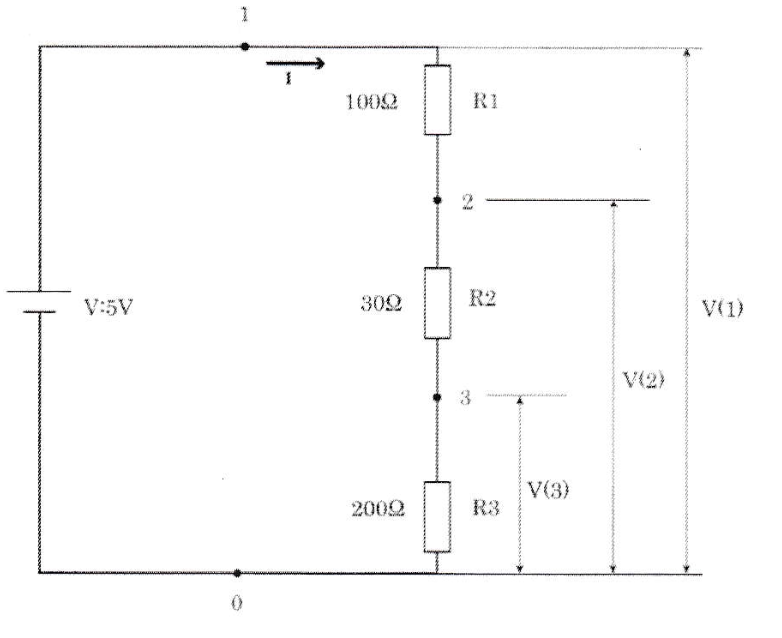
\includegraphics[width=0.6\textwidth]{assets/yobiex.png}
  \caption{予備実験回路}
\end{figure}

\begin{table}[H]
  \centering
  \caption{実験結果の比較}
  \begin{tabular}{|c|c|c|c|c|c|c|}
    \hline
    確認項目 & \( V(1) \) [V] & \( V(2) \) [V] & \( V(3) \) [V] & \( I \) [mA] & \( V_{12} \) & \( V_{23} \) \\ \hline
    実測値 & 5.00 & 3.48 & 3.05 & 14.17 & 1.52 & 0.43 \\ \hline
    シミュレーション結果 & 5.00 & 3.48 & 3.03 & 15.15 & 1.52 & 0.45 \\ \hline
    理論値(計算値) & 5.00 & 3.48 & 3.03 & 15.15 & 1.52 & 0.45 \\ \hline
    誤差率(%) & 0.00 & 0.00 & 0.6 & 0.0 & 0.0 & 4.4 \\ \hline
  \end{tabular}
\end{table}

\subsection{線形抵抗回路解析}
図3.2に示した回路を構築し、8.2節に記載したネットリストを用いてSPICEでシミュレーションを実行した結果を基に、表3.2を作成した。

\begin{figure}[H]
  \centering
  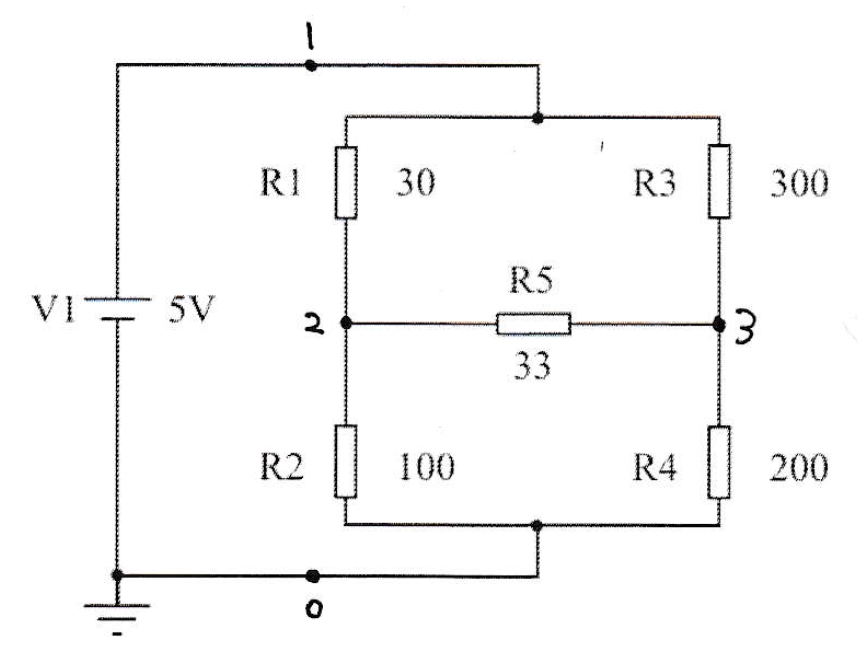
\includegraphics[width=0.6\textwidth]{assets/senkeikairo.png}
  \caption{線形抵抗回路}
\end{figure}

\begin{table}[H]
  \centering
  \caption{実験結果の比較}
  \begin{tabular}{|c|c|c|c|c|}
    \hline
    確認項目 & \( V(1) \) [V] & \( V(2) \) [V] & \( V(3) \) [V] & \( I \) [mA] \\ \hline
    実測値 & 5.00 & 3.53 & 3.23 & 45.4 \\ \hline
    シミュレーション結果 & 5.00 & 3.60 & 3.26 & 52.3 \\ \hline
    誤差率(%) & 0.0 & 1.9 & 0.9 & 13.2 \\ \hline
  \end{tabular}
\end{table}

\subsection{非線形抵抗回路解析}
図3.3に示した回路を構築し、8.3節に記載したネットリストを用いてSPICEでシミュレーションを実行した結果を基に、表3.3を作成した。

\begin{figure}[H]
  \centering
  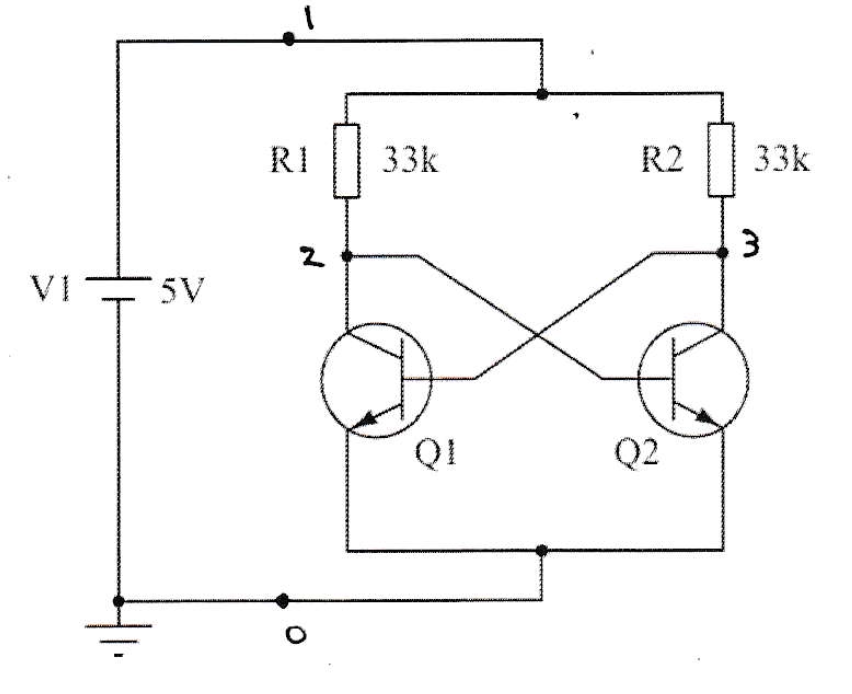
\includegraphics[width=0.6\textwidth]{assets/hisenkeikairo.png}
  \caption{非線形抵抗回路}
\end{figure}

\begin{table}[H]
  \centering
  \caption{実験結果の比較}
  \begin{tabular}{|c|c|c|c|c|}
    \hline
    確認項目 & \( V(1) \) [V] & \( V(2) \) [V] & \( V(3) \) [V] & \( I \) [mA] \\ \hline
    実測値 & 5.00 & 0.645 & 0.017 & 0.27 \\ \hline
    シミュレーション結果 & 5.00 & 0.603 & 0.603 & 0.267\\ \hline
    誤差率(%) & 0.0 & 6.97 & 97.2 & 1.1 \\ \hline
  \end{tabular}
\end{table}

\subsection{DC解析}
図3.4に示した回路を作成し、V2の電圧を0.1Vから5.0Vまで変化させたときの電流Iを測定することで表3.4を作成した。また、8.4節に記載したネットリストを用いてSPICEでシミュレーションを実行し作成したグラフを図3.5に示す。

\begin{figure}[H]
  \centering
  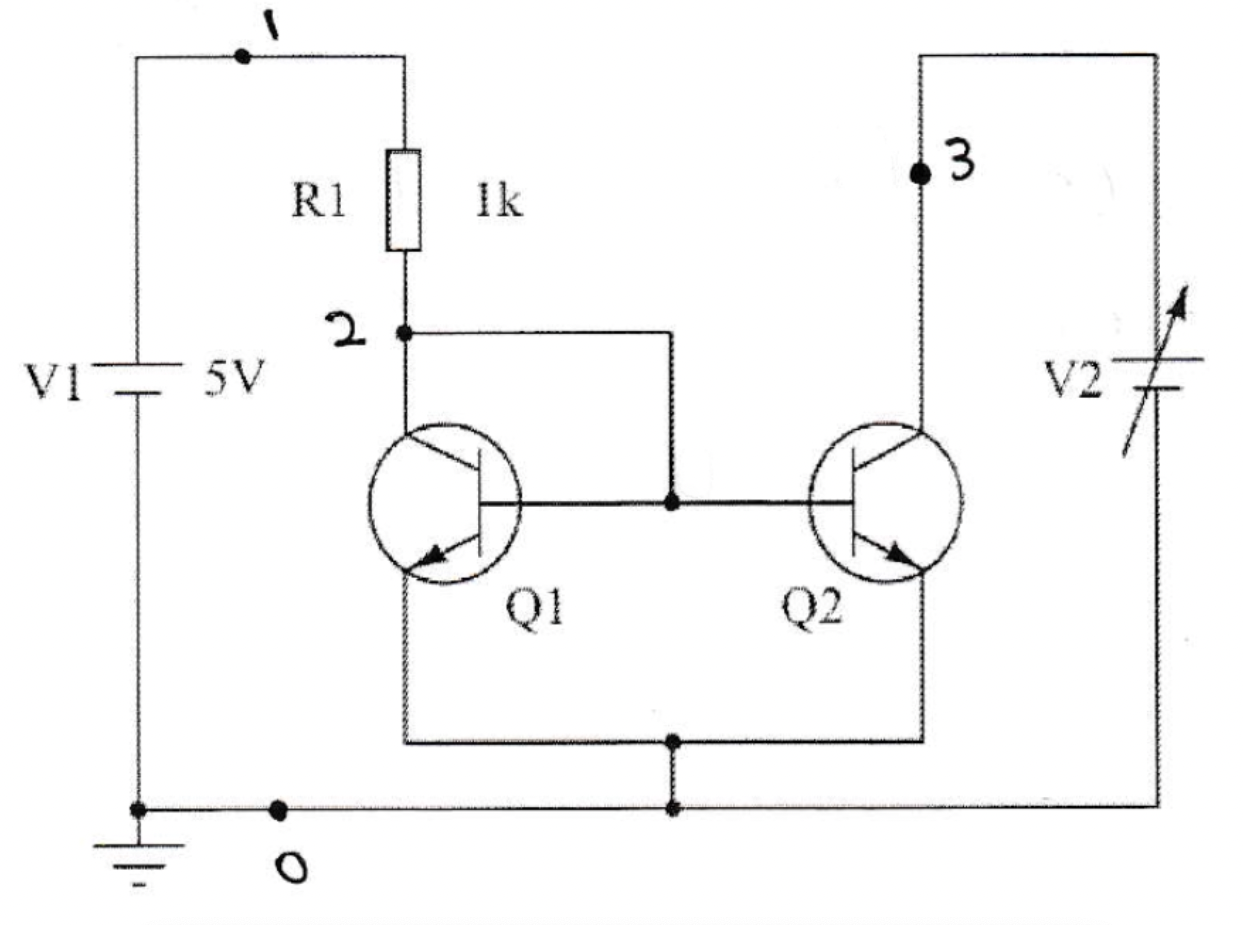
\includegraphics[width=0.6\textwidth]{assets/dckairo.png}
  \caption{DC解析回路}
\end{figure}

\begin{table}[H]
  \centering
    \caption{実験結果}
    \begin{tabular}{|c|c|c|c|c|c|c|c|c|c|c|}
      \hline
      \( V_{2} \) [V] & 0.1 & 0.2 & 0.4 & 0.6 & 0.8 & 1.0 & 2.0 & 3.0 & 4.0 & 5.0 \\ \hline
      \( I \) [mA] & 4.08 & 4.08 & 4.08 & 4.08 & 4.08 & 4.08 & 4.09 & 4.09 & 4.10 & 4.10 \\ \hline
    \end{tabular}
\end{table}

\begin{figure}[H]
  \centering
  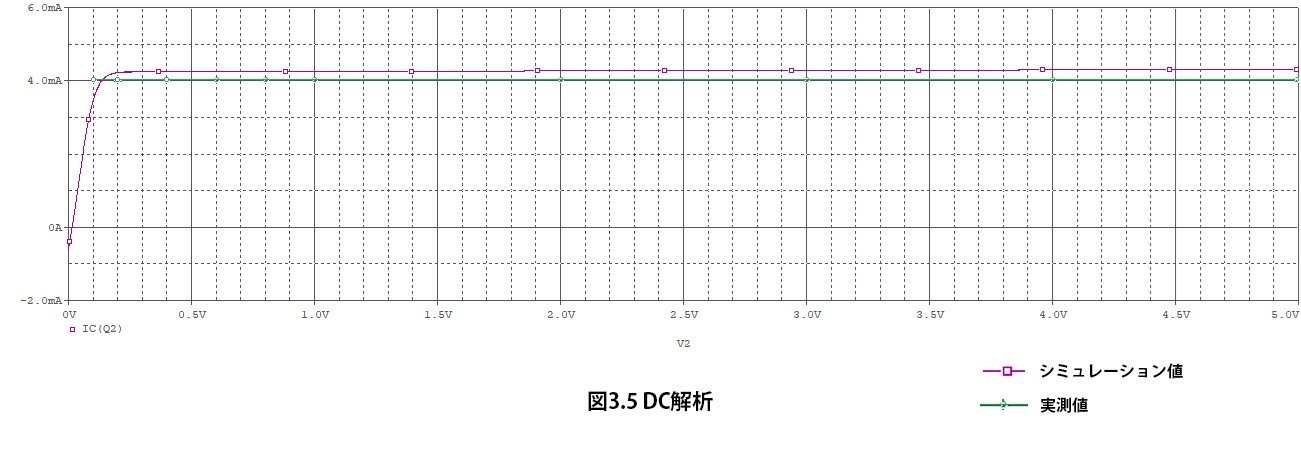
\includegraphics[width=\textwidth]{assets/dckaisekiplot.png}
  \caption{DC解析}
\end{figure}

\subsection{AC解析}
図3.6に示した回路を作成し、V1の周波数を20Hzから100kHzまで変化させたときのノード4(Vout)の電圧を測定した結果をもとに表3.5を作成した。また、8.5節に記載したネットリストを用いてSPICEでシミュレーションを実行し、さらに実測値をプロットし作成したグラフを図3.7に示す。

\begin{figure}[H]
  \centering
  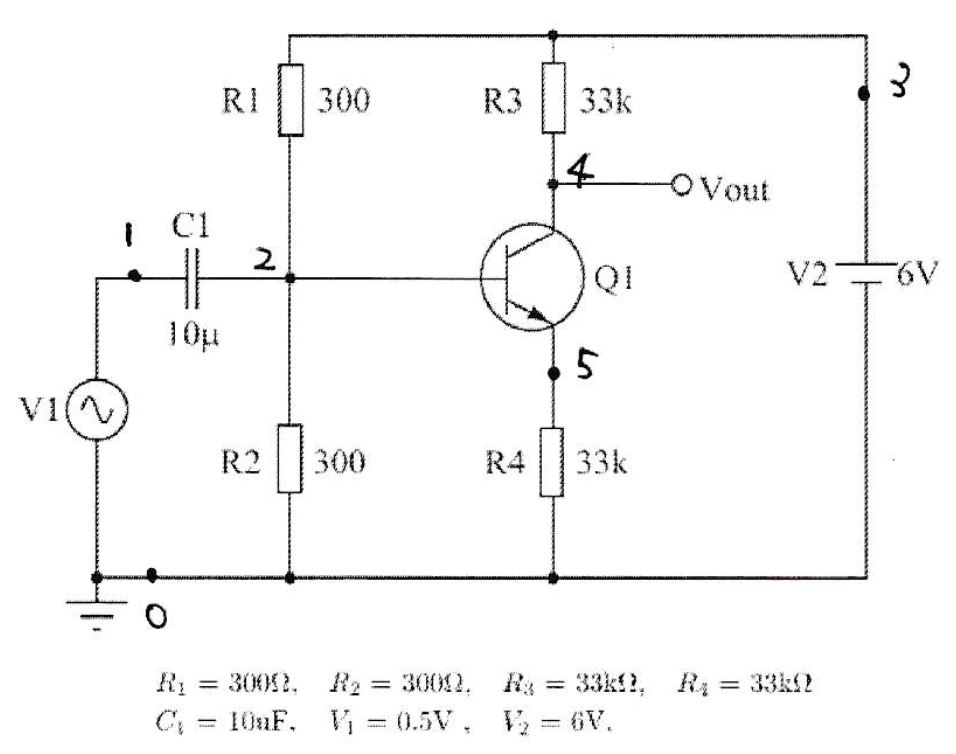
\includegraphics[width=0.7\textwidth]{assets/ackaisekikairo.png}
  \caption{AC解析回路}
\end{figure}

\begin{table}[H]
  \centering
    \caption{AC解析結果}
    \begin{tabular}{|c|c|c|c|c|c|c|c|c|c|}
      \hline
      周波数 [Hz] & 20Hz & 30Hz & 100Hz & 300Hz & 1kHz & 3kHz & 10kHz & 30kHz & 100kHz \\ \hline
      電圧 [mV] & 400 & 400 & 600 & 600 & 600 & 1000 & 1000 & 1000 & 860 \\ \hline
    \end{tabular}
\end{table}

\begin{figure}[H]
  \centering
  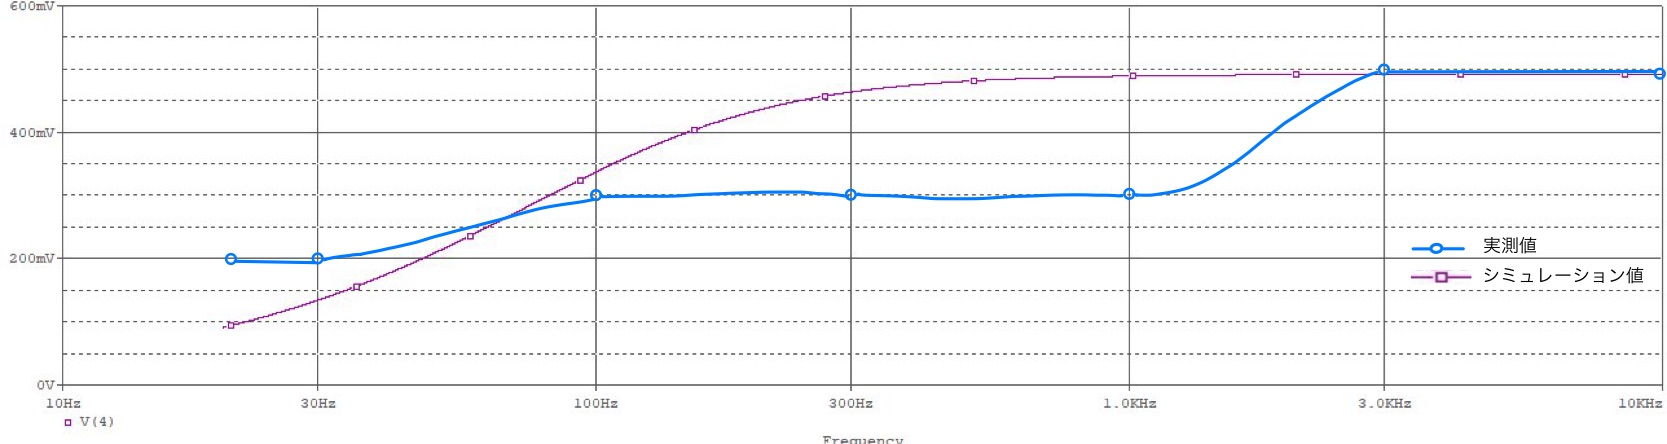
\includegraphics[width=\textwidth]{assets/ackaisekiplot.jpg}
  \caption{AC解析}
\end{figure}

\subsection{過渡解析}
図3.8に示した回路を作成し、ノード2(V)の電圧を測定した結果をもとに表3.6を作成した。オシロスコープでの観測波形を図3.9に示す。なお、周期のはじまりの電位を0V基準かつ時刻t=0とし、そこからのΔVの値を記録した。また、8.6節に記載したネットリストを用いてSPICEでシミュレーションを実行し、さらに実測値をプロットし作成したグラフを図3.10に示す。

\begin{figure}[H]
  \centering
  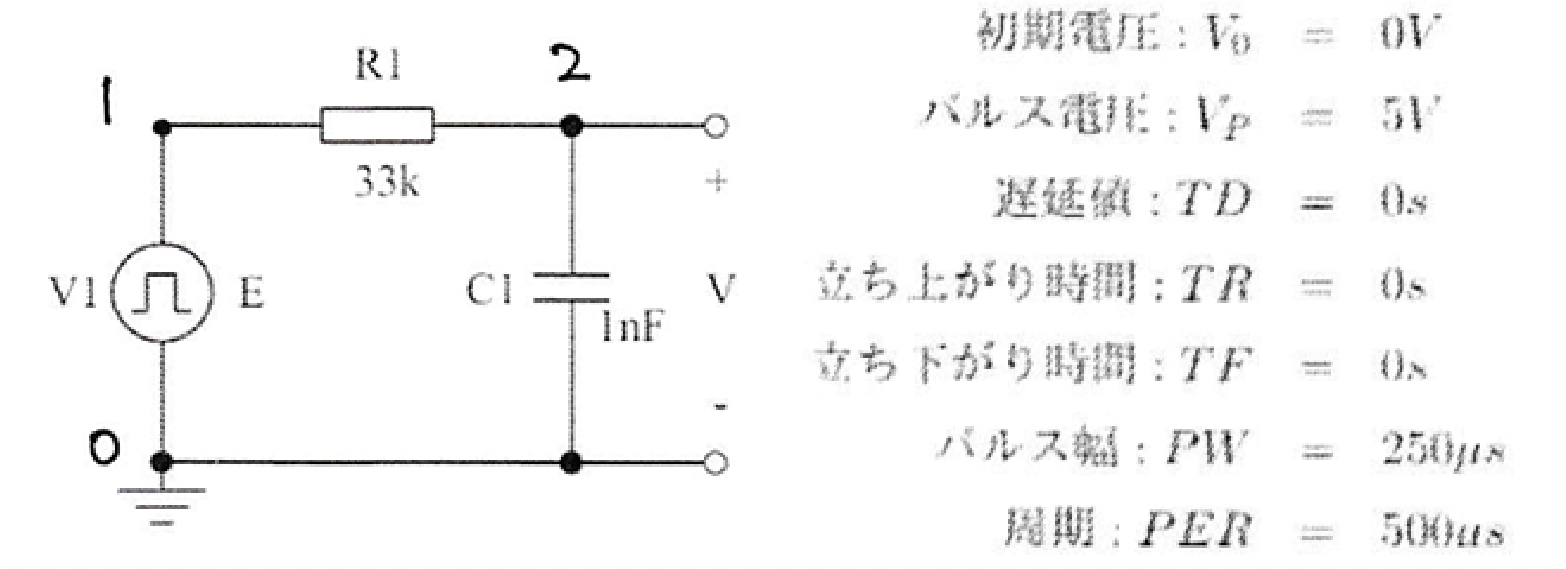
\includegraphics[width=0.8\textwidth]{assets/katokaisekikairo.png}
  \caption{過渡解析回路}
\end{figure}

\begin{table}[H]
  \centering
  \caption{過渡解析結果}
  \begin{tabular}{|c|c|c|c|c|c|c|c|}
    \hline
    \( t \) [\(\mu\)s] & 0 & 50 & 100 & 150 & 200 & 250 & 300 \\ \hline
    \( V \) [V] & 0 & 3.84 & 4.64 & 4.72 & 5.04 & 5.12 & 1.12 \\ \hline
  \end{tabular}
\end{table}

\begin{figure}[H]
  \centering
  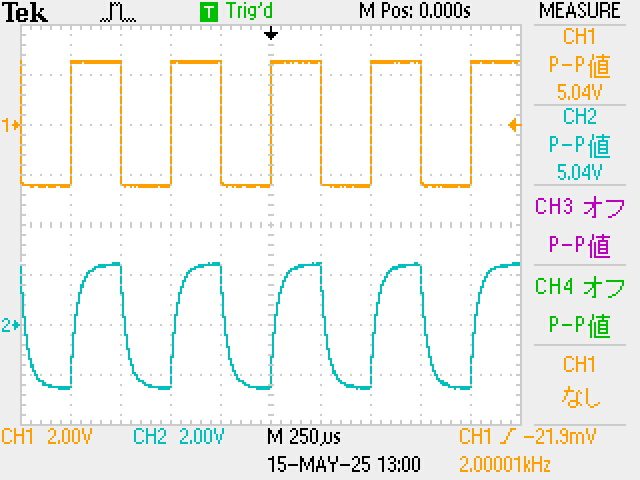
\includegraphics[width=0.5\textwidth]{assets/katooshiro.JPG}
  \caption{オシロスコープでの観測波形}
\end{figure}

\begin{figure}[H]
  \centering
  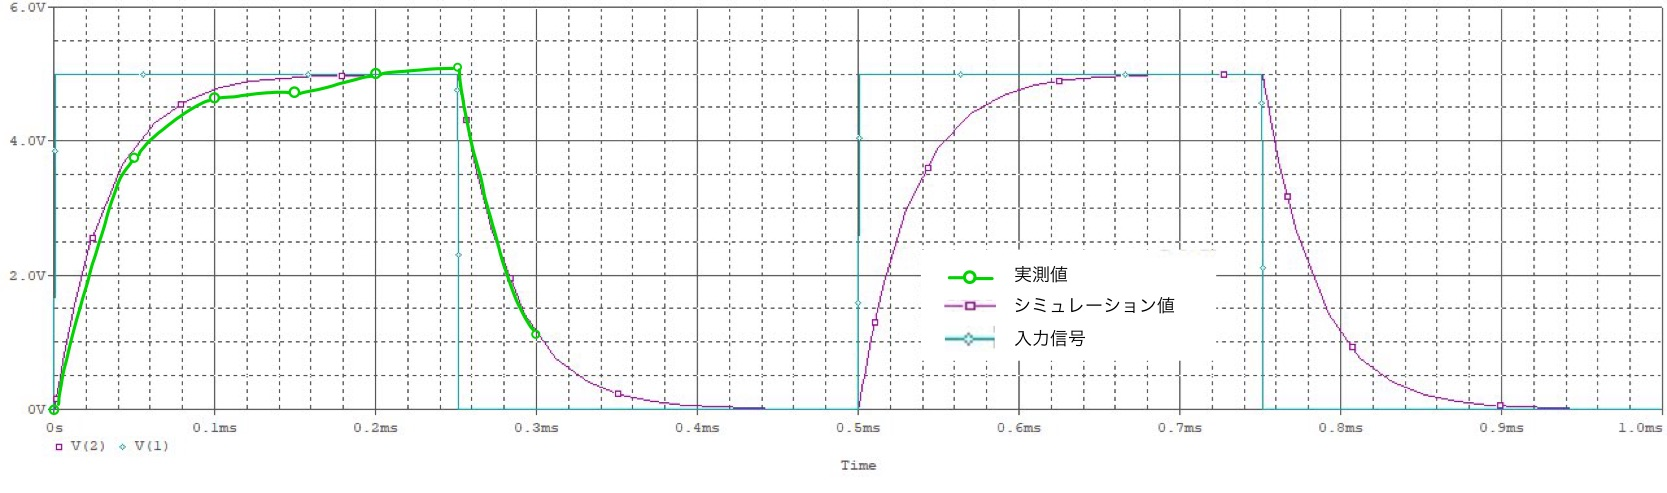
\includegraphics[width=\textwidth]{assets/katokaisekiplot.jpg}
  \caption{過渡解析}
\end{figure}

\section{考察}
\subsection{線形抵抗回路解析}
V1, V2, V3に関しては、シミュレーション値と実測値に大きな誤差は現れなかった。軽度の誤差は電圧計の測定精度等によるものだと考えられる。\\
電流値に関しては13%程度の誤差が確認され、電流計の内部抵抗によるものであると考えられる。電流計の内部抵抗を \( R_m \) とすると、測定される電流 \( I_m \) は以下のように表される。

\[
I_m = \frac{V}{R + R_m}
\]

ここで、 \( R \) は回路の抵抗、 \( V \) は電源電圧である。内部抵抗 \( R_m \) が無視できない場合、実際の電流 \( I \) よりも小さい値が測定されるため、誤差が生じる。この理論と実際の計測結果は一致する。
今回、5.0Vの電圧を加えてシミュレーションでは \( I = 52.3 \, \mathrm{mA} \) より、抵抗値 \( R \) は以下のように計算される。

\[
R \approx \frac{V}{I} = \frac{5.0}{0.0523} \approx 95.6 \, \Omega
\]

一方、実測値では \( I = 45.4 \, \mathrm{mA} \) より、回路全体の抵抗値 \( R + R_m \) は以下のように計算される。

\[
R + R_m \approx \frac{V}{I} = \frac{5.0}{0.0454} \approx 110.1 \, \Omega
\]

これらの結果から、電流計の内部抵抗 \( R_m \) は以下のように求められる。

\[
R_m \approx 110.1 - 95.6 \approx 15 \, \Omega
\]

したがって、電流計の内部抵抗 \( R_m \) は約 \( 15 \, \Omega \) であると考えられる。

\subsection{非線形抵抗回路解析}
V1,V2,Iに関してはシミュレーション結果と概ね一致しているといえるが、V3に関しては実測値がシミュレーション結果より極端に小さくなっていることがわかる。\\

\paragraph{コレクタ電圧の初期値を設定した場合のシミュレーション}
図3.3の回路において、Q1のコレクタ電圧の初期値を設定した場合のシミュレーション結果を表4.1に示す。またシミュレーションで使用したネットリストを8.3節に示す。
\begin{table}[H]
  \centering
  \caption{非線形抵抗回路解析シミュレーション結果}
  \begin{tabular}{|c|c|c|c|c|}
    \hline
    初期値 [V] & \( V(1) \) [V] & \( V(2) \) [V] & \( V(3) \) [V] & \( I \) [mA] \\ \hline
    0.2 & 5.00 & 0.238 & 0.644 & 0.283 \\ \hline
    0.6 & 5.00 & 0.603 & 0.603 & 0.267 \\ \hline
    0.8 & 5.00 & 0.644 & 0.238 & 0.283 \\ \hline
  \end{tabular}
\end{table}

コレクタ電圧を0.6Vとしたときは、初期値を設定しなかったときとシミュレーション結果は変化しなかったが、初期値を0.2VとしたときにはV2の低下かつV3の増加、0.8VとしたときにはV2の増加かつV3の低下が対称的にみられた。

この主な要因として、SPICEシミュレーションでは非線形回路方程式の解法にニュートン法が用いられていることが挙げられる。非線形回路には複数の解(動作点)が存在し、安定解と不安定解が混在する。ニュートン法は初期値の設定によって収束する解が変わるため、実験と異なる動作点に収束する場合がある。今回のシミュレーションでは、コレクタ電圧の初期値を変えることでV2とV3の値が対称的に変化する現象が見られ、これは非線形系特有の多重解や双安定性が影響していると考えられる。(4)(5)

\subsection{DC解析}
シミュレーションでは値が一定であるのに対し、実測値では電圧が上がるにつれてわずかに電流値も大きくなっていることが確認された。

この現象の主な原因として考えられるのは、実際のトランジスタにおける「アーリー効果」である。アーリー効果とは、トランジスタのコレクタ-エミッタ間電圧 (VCE) が増加すると、実効的なベース幅が減少し、その結果コレクタ電流がわずかに増加する現象である。シミュレーションでは理想的なトランジスタモデルが使用されている可能性があり、このアーリー効果が十分に考慮されていないことが原因と考えられる。(6)

\subsection{AC解析}
実験値はシミュレーション値と異なり、100kHz付近で電圧が減少している。この原因として、プローブの影響が考えられる。プローブには寄生容量 \( C \) と抵抗 \( R \) が存在し、これらが回路に並列に接続されることで、回路全体の周波数特性に影響を与える。

今回の実験では、プローブの寄生容量や回路インピーダンスの影響により、100kHz付近で信号の減衰が顕著になったと考えられる。ここで、カットオフ周波数 \( f_c \) が約100kHzであると仮定すると、時定数であるRC積は次式で逆算できる。

\[
RC = \frac{1}{2\pi f_c}
\]

したがって、

\[
RC = \frac{1}{2\pi \times 1.0 \times 10^5} \approx 1.59\,\mu\mathrm{s}
\]

となる。

一方、シミュレーションでは理想的な条件が仮定されているため、プローブの影響が考慮されず、減衰が見られなかったと考えられる。(7)

\subsection{過渡解析}
本実験において、図3.10よりコンデンサの充電過程に関するシミュレーション結果では約 $200\,\mu\mathrm{s}$ 時点で電圧が定常状態に達したとみなされていると読み取れる。一方、実測データでは $250\,\mu\mathrm{s}$ 程度までわずかに電圧が上昇し続ける様子が観測された。

RC回路におけるコンデンサの電圧変化は
\[
V(t) = E\left(1 - e^{-t/RC}\right)
\]
であり、理論的には $t \to \infty$ のとき初めて $V(t) = E$ に達する。つまり、このプロセスは有限時間内に完結することはなく、常に漸近的に平衡状態へと近づく挙動を示す。

シミュレーションでは、電圧が起電力 $E$ の 99\% または 99.9\% に達した時点で「定常状態」とみなされることが多く、これにより $200\,\mu\mathrm{s}$ 付近で電圧の変化が打ち切られる。しかし、実測値ではこうした近似を行わないため、指数関数的にわずかに残る電圧上昇が $250\,\mu\mathrm{s}$ 付近まで可視化されると考えられる。(8)

また、プローブの寄生容量や内部抵抗などによっても時定数に影響が出ると考えられる。

さらに、詳しくは5.1節で言及するが、シミュレーターが使用している数値計算法の誤差も大きな要因として考えられる。

\section{追加課題}

\subsection{過渡解析の各種数値計算法比較}
ここでは、RC回路の過渡応答を数値的に計算する。$0$から$300\,\mu\mathrm{s}$の範囲で、前進オイラー法、後退オイラー法、台形法を用いてシミュレーションを行う。

厳密解について、RC回路の微分方程式は次式で表される。
\[
i(t) = C \frac{dv_C}{dt}
\]
また、オームの法則より
\[
i(t) = \frac{E - v_C(t)}{R}
\]
したがって、これらを連立すると
\[
C \frac{dv_C}{dt} = \frac{E - v_C(t)}{R}
\]
\[
\frac{dv_C}{dt} + \frac{1}{RC} v_C(t) = \frac{E}{RC}
\]

この微分方程式の厳密解は、初期条件 \( v_C(0) = 0 \) のもとで
\[
v_C(t) = E \left( 1 - e^{- \frac{t}{RC}} \right)
\]
となる。

2.4節より、各数値解析法による計算をした結果を表5.1に示す。
各手法の差分方程式は以下のようになる。

\begin{enumerate}
  \item \textbf{前進オイラー法}
  \[
    v_{n+1} = v_n + \frac{h}{RC}(V_0 - v_n)
  \]
  \item \textbf{後退オイラー法}
  \[
    v_{n+1} = \frac{V_0 h + RC v_n}{h + RC}
  \]
  \item \textbf{台形法}
  \[
    v_{n+1} = \frac{2 V_0 h + 2 (RC - h) v_n}{h + 2RC}
  \]
\end{enumerate}

ここで、\( h \) は時間刻み幅、\( RC \) は回路の時定数、\( V_0 \) は入力電圧である。

今回 \( h = 50 \, \mu\mathrm{s}, V_0 = 5 \, \mathrm{V}, C = 1 \, \mathrm{nF}, R = 33 \, \mathrm{k}\Omega \) を代入して計算する。
それぞれの計算結果を表5.1に示す。

\begin{table}[H]
  \centering
  \caption{各手法による計算結果}
  \begin{tabular}{|c|c|c|c|c|c|c|c|}
    \hline
    時間 [\(\mu\)s] & 0 & 50 & 100 & 150 & 200 & 250 & 300 \\ \hline
    厳密解 [V] & 0.000 & 3.90 & 4.76 & 4.95 & 4.99 & 5.00 & 5.00 \\ \hline
    前進オイラー [V] & 0.000 & 7.58 & 3.67 & 5.68 & 4.65 & 5.18 & 4.91 \\ \hline
    後退オイラー [V] & 0.000 & 3.01 & 4.21 & 4.69 & 4.88 & 4.95 & 4.98 \\ \hline
    台形法 [V] & 0.000 & 4.31 & 4.90 & 4.99 & 5.00 & 5.00 & 5.00 \\ \hline
  \end{tabular}
\end{table}

この結果より図5.1を作成した。

\begin{figure}[H]
  \centering
  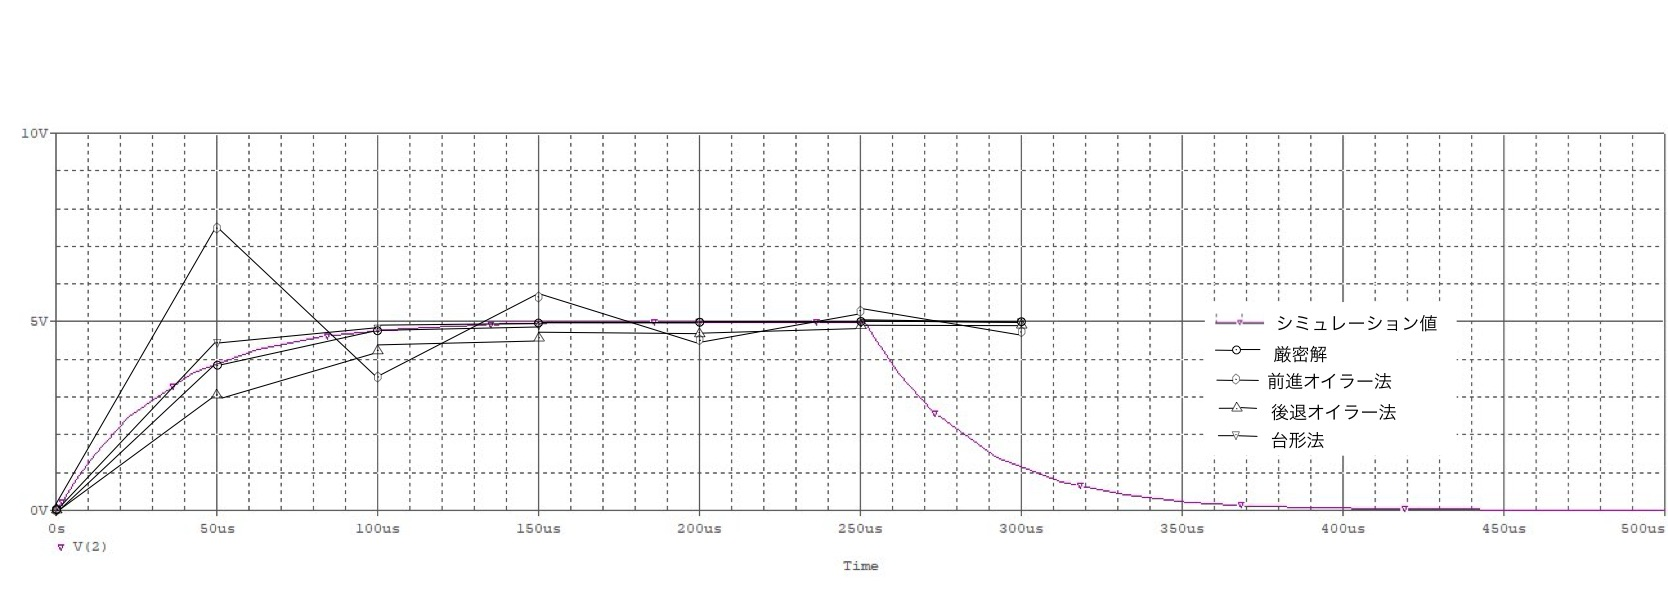
\includegraphics[width=\textwidth]{assets/katohikakuplot.jpg}
  \caption{各手法による計算結果の比較}
\end{figure}

この結果から、台形法、後退オイラー法、前進オイラー法の順に誤差が少ないことがわかる。

\subsection{フィルタ回路の作成}
\subsubsection{53Hz以上の周波数を通過させる回路(ハイパスフィルタ)}
抵抗とコンデンサを用いてカットオフ周波数を計算し、設計した回路を図5.2に示す。また、V1を1.0V(p-p値)にして周波数を5Hzから10kHzまで変化させたときのV2の実測値を表5.2にまとめ、8.7節のネットリストによるシミュレーション結果と実測値をプロットしたグラフを図5.3に示す。

\begin{figure}[H]
  \centering
  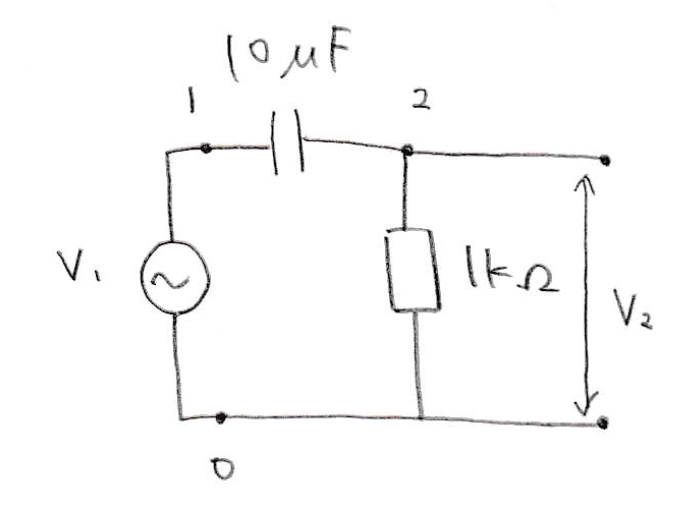
\includegraphics[width=0.6\textwidth]{assets/highpasskairo.png}
  \caption{ハイパスフィルタ回路}
\end{figure}

\begin{table}[H]
  \centering
  \caption{ハイパスフィルタ実測値}
  \begin{tabular}{|c|c|c|c|c|c|c|c|c|c|c|c|}
    \hline
    周波数 [Hz] & 5 & 10 & 20 & 50 & 100 & 200 & 500 & 1k & 2k & 5k & 10k \\ \hline
    電圧 [mV] & 100 & 240 & 720 & 960 & 1000 & 1000 & 1000 & 1000 & 1000 & 1000 & 1000 \\ \hline
  \end{tabular}
\end{table}

\begin{figure}[H]
  \centering
  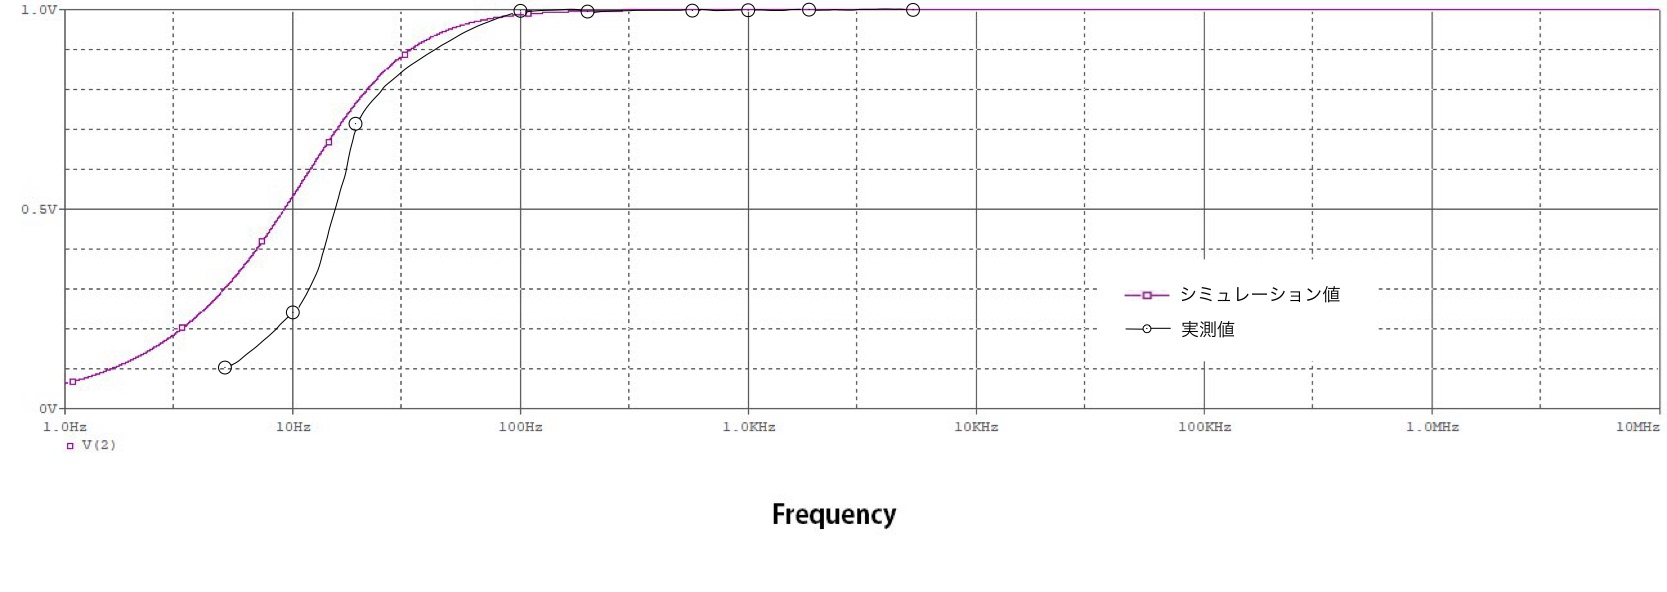
\includegraphics[width=\textwidth]{assets/highpass.jpg}
  \caption{シミュレーション結果}
\end{figure}

\subsubsection{160kHz以下の周波数を通過させる回路(ローパスフィルタ)}
抵抗とコンデンサを用いてカットオフ周波数を計算し、設計した回路を図5.4に示す。また、V1を1.0V(p-p値)にして周波数を5kHzから1MHHzまで変化させたときのV2の実測値を表5.3にまとめ、8.8節のネットリストによるシミュレーション結果と実測値をプロットしたグラフを図5.5に示す。

\begin{figure}[H]
  \centering
  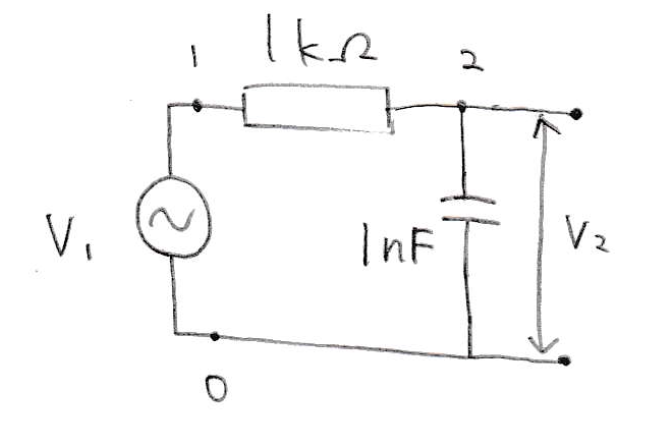
\includegraphics[width=0.6\textwidth]{assets/lowpasskairo.png}
  \caption{ローパスフィルタ回路}
\end{figure}

\begin{table}[H]
  \centering
  \caption{ローパスフィルタ実測値}
  \begin{tabular}{|c|c|c|c|c|c|c|c|}
    \hline
    周波数 [kHz] & 5 & 10 & 50 & 100 & 200 & 500 & 1000 \\ \hline
    電圧 [mV] & 1000 & 1000 & 1000 & 900 & 680 & 380 & 240 \\ \hline
  \end{tabular}
\end{table}

\begin{figure}[H]
  \centering
  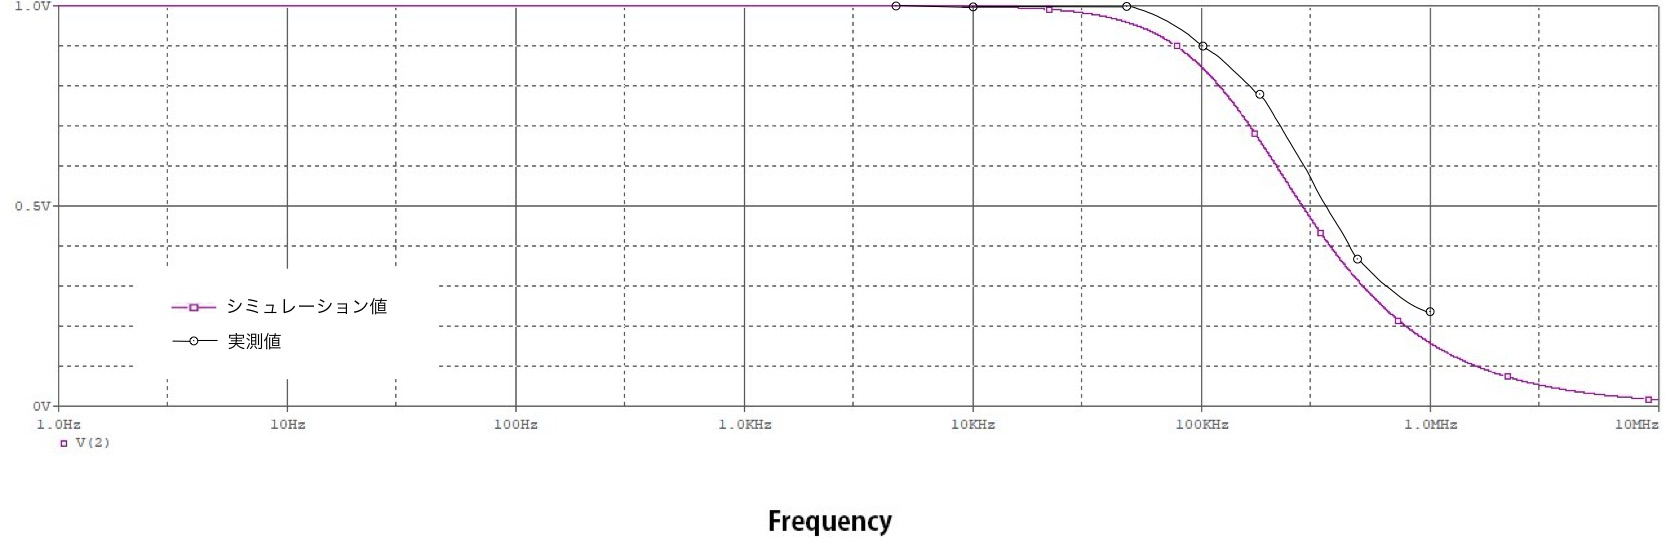
\includegraphics[width=\textwidth]{assets/lowpass.jpg}
  \caption{シミュレーション結果}
\end{figure}

\subsubsection{53Hz以上かつ160kHz以下の周波数を通過させる回路(バンドパスフィルタ)}
抵抗とコンデンサを用いてカットオフ周波数を計算し、設計した回路を図5.6に示す。また、V1を1.0V(p-p値)にして周波数を5Hzから1MHHzまで変化させたときのV2の実測値を表5.4にまとめ、8.9節のネットリストによるシミュレーション結果と実測値をプロットしたグラフを図5.7に示す。

\begin{figure}[H]
  \centering
  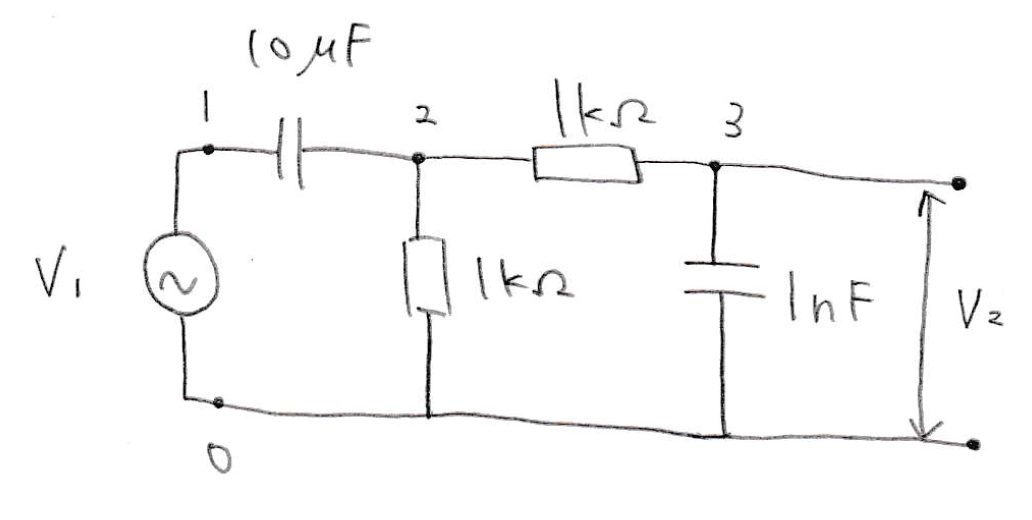
\includegraphics[width=0.6\textwidth]{assets/bandpasskairo.png}
  \caption{バンドパスフィルタ回路}
\end{figure}

\begin{table}[H]
  \centering
    \caption{バンドパスフィルタ実測値}
    \begin{tabular}{|c|c|c|c|c|c|c|c|c|c|}
      \hline
      周波数 [Hz] & 5 & 10 & 20 & 50 & 100 & 200 & 500 & 1k & 2k \\ \hline
      電圧 [mV] & 184 & 528 & 744 & 896 & 920 & 936 & 980 & 980 & 1000 \\ \hline
      \hline
      周波数 [Hz] & 5k & 10k & 20k & 50k & 100k & 200k & 500k & 1M & - \\ \hline
      電圧 [mV] & 1000 & 1000 & 1000 & 960 & 820 & 640 & 380 & 220 & - \\ \hline
    \end{tabular}
\end{table}

\begin{figure}[H]
  \centering
  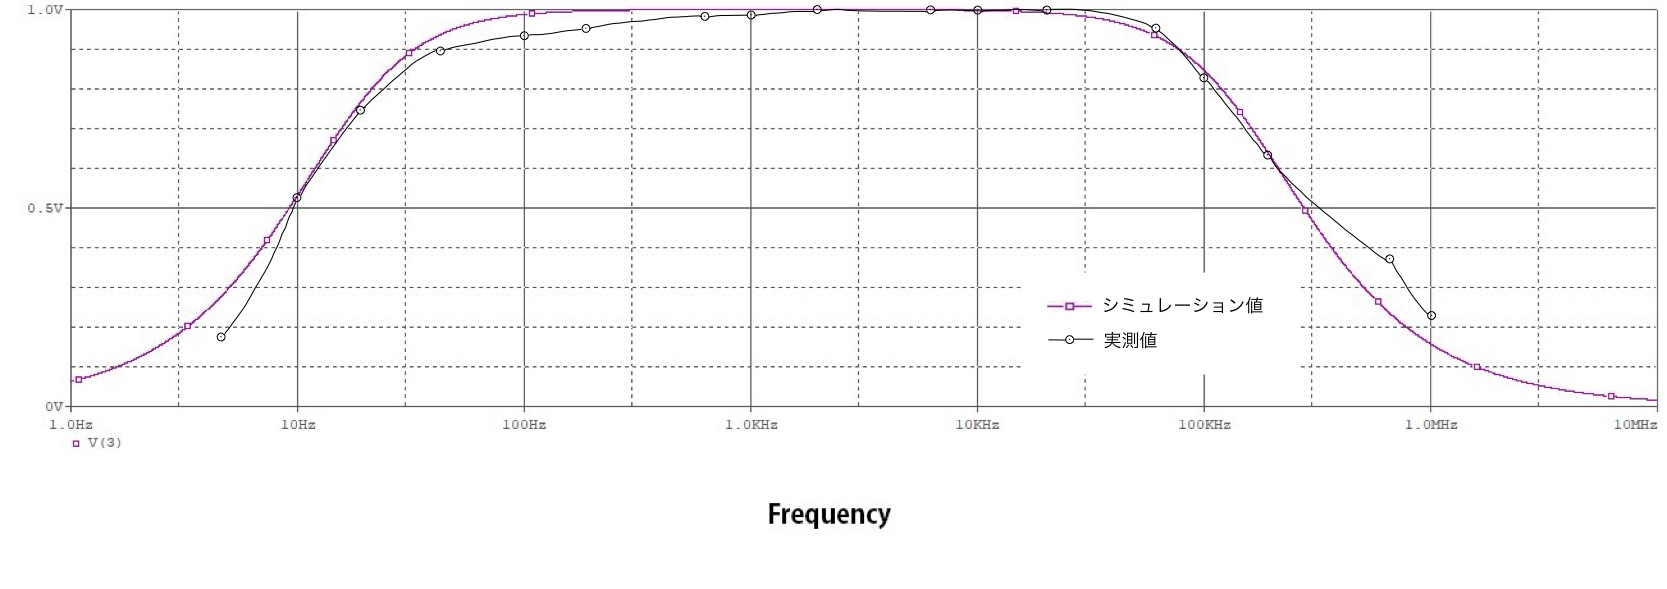
\includegraphics[width=\textwidth]{assets/bandpass.jpg}
  \caption{シミュレーション結果}
\end{figure}

概ねシミュレーション結果と同様の実測値が得られた。

\section{使用機材}
表6.1に示す。
\begin{table}[H]
  \centering
  \caption{使用機材一覧}
  \begin{tabular}{|c|c|c|c|}
    \hline
    名称 & 型式 & 製造元 & 管理番号 \\ \hline
    直流電流源 & PMC35-1.2DU & KIKUSUI & UK002986 \\ \hline
    ファンクションジェネレータ & FG-274 & TEXIO & 17073061 \\ \hline
    オシロスコープ & TDS 2004B & Tektronix & C100578 \\ \hline
    デジタルマルチメータ & CD731 & Sanwa & 0152985 \\ \hline
  \end{tabular}
\end{table}

\section{参考文献}
\begin{enumerate}
  \item SPICEとは, 電子回路シミュレーションの基礎 \\
    \url{https://techweb.rohm.co.jp/product/simulation/7688/}\\
    閲覧日:2025年5月17日
  \item アナログ電子回路シミュレータのメリット・デメリット \\
    \url{https://spiceman.jp/circuit-simulator-merit-demerit/}\\
    閲覧日:2025年5月17日
  \item 長尾佑紀, 『数値計算の常識を変える! 安定性で選ぶ常微分方程式の数値解法』, 共立出版, 2022年.
  \item SPICE におけるニュートン法の課題と対策\\
  \url{https://qiita.com/sukimaengineer/items/0dbce87dc5fb2c17aeb5} \\
  閲覧日:2025年5月19日
   \item LTspiceの優位性\\
  \url{https://www.analog.com/jp/resources/technical-articles/spice-differentiation.html} \\
  閲覧日:2025年5月19日
  \item アーリー効果とは?メカニズムとアーリー電圧の求め方, Analogista \\
  \url{https://analogista.jp/early-effect/} \\
  閲覧日:2025年5月19日
  \item プローブの基礎, YOKOGAWA \\
  \url{https://tmi.yokogawa.com/jp/library/resources/measurement-tips/probe_basics/} \\
  閲覧日:2025年5月19日
  \item コンデンサの役割を学ぶ, APS, 組み込み氷解専門メディア \\
  \url{https://www.aps-web.jp/academy/ec/188/} \\
  閲覧日:2025年5月19日
\end{enumerate}

\section{付録}
本実験のシミュレーションで使用したSPICEのネットリストを以下に示す。

なお、今回の実験で使用したトランジスタのモデル定義については以下であり、各節では省略している。
\begin{verbatim}
.MODEL     SC1815Y-1  NPN  (                  is   = 9.37282E-15  
   + bf    = 170.4435407  nf   = 0.9950205    vaf  = 289.6037168  
   + ikf   = 0.8720864    ise  = 1.60756E-15  ne   = 1.5936166 
   + br    = 5.0638521    nr   = 0.9955386    var  = 15.8262796  
   + ikr   = 2.33473E-3   isc  = 9.62491E-15  nc   = 1.0344131  
   + rb    = 55           re   = 0.8331605    rc   = 0.7956197  
   + cje   = 1.48343E-11  vje  = 0.544257     mje  = 0.2984869  
   + tf    = 5.3964E-10   xtf  = 0.1584639    vtf  = 5.843019  
   + itf   = 1.48869E-3   cjc  = 4.62178E-12  vjc  = 0.440088  
   + mjc   = 0.3482488    fc   = 0.8176782	 )
\end{verbatim}

\subsection{予備実験回路解析}
\begin{verbatim}
Pre Ex
V 1 0 5V
R1 1 2 100
R2 2 3 30
R3 3 0 200
.OP
.END
\end{verbatim}

\subsection{線形抵抗回路解析}
\begin{verbatim}
Linear Analye
V 1 0 5V
R1 1 2 30
R2 2 0 100
R3 1 3 300
R4 3 0 200
R5 2 3 33
.OP
.END
\end{verbatim}

\subsection{非線形抵抗回路解析}
\subsubsection{コレクタ電圧の初期値設定なし}
\begin{verbatim}
Non-linear Analyze
V 1 0 5V
R1 1 2 33k
R2 1 3 33k
Q1 2 3 0 SC1815Y-1
Q2 3 2 0 SC1815Y-1
.OP
.END
\end{verbatim}

\subsubsection{コレクタ電圧の初期値を0.2Vに設定}
\begin{verbatim}
Non-linear Analyze 0.2
V 1 0 5V
R1 1 2 33k
R2 1 3 33k
Q1 2 3 0 SC1815Y-1
Q2 3 2 0 SC1815Y-1
.nodeset V(2) 0.2
.OP
.END
\end{verbatim}

\subsubsection{コレクタ電圧の初期値を0.6Vに設定}
\begin{verbatim}
Non-linear Analyze 0.6
V 1 0 5V
R1 1 2 33k
R2 1 3 33k
Q1 2 3 0 SC1815Y-1
Q2 3 2 0 SC1815Y-1
.nodeset V(2) 0.6
.OP
.END
\end{verbatim}

\subsubsection{コレクタ電圧の初期値を0.8Vに設定}
\begin{verbatim}
Non-linear Analyze 0.8
V 1 0 5V
R1 1 2 33k
R2 1 3 33k
Q1 2 3 0 SC1815Y-1
Q2 3 2 0 SC1815Y-1
.nodeset V(2) 0.8
.OP
.END
\end{verbatim}

\subsection{DC解析}
\begin{verbatim}
DC Analyze
V1 1 0 5V
V2 3 0 5V
R1 1 2 1k
Q1 2 2 0 SC1815Y-1
Q2 3 2 0 SC1815Y-1
.DC V2 0 5 1m
.PROBE
.END
\end{verbatim}

\subsection{AC解析}
\begin{verbatim}
AC Analyze
V1 1 0 AC 0.5V
V2 3 0 6V
C1 1 2 10uF
R1 2 3 300
R2 2 0 300
R3 3 4 33k
R4 5 0 33k
Q1 4 2 5 SC1815Y-1
.AC DEC 49999 20Hz 100kHz
.PROBE
.END
\end{verbatim}

\subsection{過渡解析}
\begin{verbatim}
Transient Analyze
V1 1 0 PULSE(0 5 0 0 0 250u 500u)
R1 1 2 33k
C1 2 0 1n
.TRAN 1u 1m
.PROBE
.END
\end{verbatim}

\subsection{ハイパスフィルタ}
\begin{verbatim}
High Pass Filter
V1 1 0 AC 1V
R1 2 0 1k
C1 1 2 10u
.AC DEC 10000 1Hz 10000kHz
.PROBE
.END
\end{verbatim}

\subsection{ローパスフィルタ}
\begin{verbatim}
Low Pass Filter
V1 1 0 AC 1V
R1 1 2 1k
C1 2 0 1n
.AC DEC 10000 1Hz 10000kHz
.PROBE
.END
\end{verbatim}

\subsection{バンドパスフィルタ}
\begin{verbatim}
Band Pass Filter
V1 1 0 AC 1V
C1 1 2 10u
R1 2 0 1k
R2 2 3 1k
C2 3 0 1n
.AC DEC 10000 1Hz 10000kHz
.PROBE
.END
\end{verbatim}

\end{document}